\documentclass[12pt]{article}
\usepackage[margin=2cm]{geometry}
\usepackage{cite}
\usepackage{float}
\usepackage{graphicx}
\usepackage[caption=false]{subfig}
  \DeclareGraphicsExtensions{.png}
\usepackage{amsmath}
\usepackage{amsfonts}
\usepackage{url}
\usepackage{tikz}
\usetikzlibrary{shapes,arrows}
\usepackage{bm,times}
\usepackage{pgfgantt}
\usepackage{indentfirst}
\usepackage{array}
\begin{document}

\begin{titlepage}
  \setlength{\parindent}{0pt}
  \setlength{\parskip}{0pt}

  { \Large
    Imperial College London\\[17pt]
    Department of Electrical and Electronic Engineering\\[17pt]
    Final Year Project Report (DRAFT)
  }

  \rule{\columnwidth}{3pt}
  \vfill
  \centering
  
\includegraphics[width=0.8\columnwidth]{img/placeholder.png}
  \vfill

  \begin{table}[h]
  \def\arraystretch{1.8}
    \begin{tabular}{p{40mm}p{\dimexpr\columnwidth-40mm}}
      Project Title: & \textbf{A High-radix Online Arithmetic Verification System} \\
      Student:       & \textbf{Zifan Wang} \\
      CID:           & \textbf{01077639} \\
      Course:        & \textbf{EEE4} \\
      Project Supervisor: & \textbf{Dr. James J. Davis} \\
      Second Marker: & \textbf{Dr. Christos Bouganis}
    \end{tabular}
  \end{table}
\end{titlepage}


% \markboth{2018-2019}{?}
\setcounter{tocdepth}{2}
\tableofcontents

\newpage

\begin{abstract}
  Nice abstract
\end{abstract}

\section{Introduction}
\section{Background}
  But I must explain to you how all this mistaken idea of denouncing of a pleasure and praising pain was born and I will give you a complete account of the system, and expound the actual teachings of the great explorer of the truth, the master-builder of human happiness.
No one rejects, dislikes, or avoids pleasure itself, because it is pleasure, but because those who do not know how to pursue pleasure rationally encounter consequences that are extremely painful.
Nor again is there anyone who loves or pursues or desires to obtain pain of itself, because it is pain, but occasionally circumstances occur in which toil and pain can procure him some great pleasure.
To take a trivial example, which of us ever undertakes laborious physical exercise, except to obtain some advantage from it?
But who has any right to find fault with a man who chooses to enjoy a pleasure that has no annoying consequences, or one who avoids a pain that produces no resultant pleasure?

On the other hand, we denounce with righteous indignation and dislike men who are so beguiled and demoralized by the charms of pleasure of the moment, so blinded by desire, that they cannot foresee the pain and trouble that are bound to ensue; and equal blame belongs to those who fail in their duty through weakness of will, which is the same as saying through shrinking from toil and pain. 
These cases are perfectly simple and easy to distinguish.
In a free hour, when our power of choice is untrammeled and when nothing prevents our being able to do what we like best, every pleasure is to be welcomed and every pain avoided.
But in certain circumstances and owing to the claims of duty or the obligations of business it will frequently occur that pleasures have to be repudiated and annoyances accepted.
The wise man therefore always holds in these matters to this principle of selection: he rejects pleasures to secure other greater pleasures, or else he endures pains to avoid worse.
\section{Requirements Capture}
  But I must explain to you how all this mistaken idea of denouncing of a pleasure and praising pain was born and I will give you a complete account of the system, and expound the actual teachings of the great explorer of the truth, the master-builder of human happiness.
No one rejects, dislikes, or avoids pleasure itself, because it is pleasure, but because those who do not know how to pursue pleasure rationally encounter consequences that are extremely painful.
Nor again is there anyone who loves or pursues or desires to obtain pain of itself, because it is pain, but occasionally circumstances occur in which toil and pain can procure him some great pleasure.
To take a trivial example, which of us ever undertakes laborious physical exercise, except to obtain some advantage from it?
But who has any right to find fault with a man who chooses to enjoy a pleasure that has no annoying consequences, or one who avoids a pain that produces no resultant pleasure?

On the other hand, we denounce with righteous indignation and dislike men who are so beguiled and demoralized by the charms of pleasure of the moment, so blinded by desire, that they cannot foresee the pain and trouble that are bound to ensue; and equal blame belongs to those who fail in their duty through weakness of will, which is the same as saying through shrinking from toil and pain. 
These cases are perfectly simple and easy to distinguish.
In a free hour, when our power of choice is untrammeled and when nothing prevents our being able to do what we like best, every pleasure is to be welcomed and every pain avoided.
But in certain circumstances and owing to the claims of duty or the obligations of business it will frequently occur that pleasures have to be repudiated and annoyances accepted.
The wise man therefore always holds in these matters to this principle of selection: he rejects pleasures to secure other greater pleasures, or else he endures pains to avoid worse.
\section{Analysis and Design}
  But I must explain to you how all this mistaken idea of denouncing of a pleasure and praising pain was born and I will give you a complete account of the system, and expound the actual teachings of the great explorer of the truth, the master-builder of human happiness.
No one rejects, dislikes, or avoids pleasure itself, because it is pleasure, but because those who do not know how to pursue pleasure rationally encounter consequences that are extremely painful.
Nor again is there anyone who loves or pursues or desires to obtain pain of itself, because it is pain, but occasionally circumstances occur in which toil and pain can procure him some great pleasure.
To take a trivial example, which of us ever undertakes laborious physical exercise, except to obtain some advantage from it?
But who has any right to find fault with a man who chooses to enjoy a pleasure that has no annoying consequences, or one who avoids a pain that produces no resultant pleasure?

On the other hand, we denounce with righteous indignation and dislike men who are so beguiled and demoralized by the charms of pleasure of the moment, so blinded by desire, that they cannot foresee the pain and trouble that are bound to ensue; and equal blame belongs to those who fail in their duty through weakness of will, which is the same as saying through shrinking from toil and pain. 
These cases are perfectly simple and easy to distinguish.
In a free hour, when our power of choice is untrammeled and when nothing prevents our being able to do what we like best, every pleasure is to be welcomed and every pain avoided.
But in certain circumstances and owing to the claims of duty or the obligations of business it will frequently occur that pleasures have to be repudiated and annoyances accepted.
The wise man therefore always holds in these matters to this principle of selection: he rejects pleasures to secure other greater pleasures, or else he endures pains to avoid worse.
\section{Implementation}
\section{Testing}
\section{Results}
\section{Evaluation}
\section{Conclusion}
\section{Further Work}
\section{User Guide}

\newpage
\appendix

% \section{A Brief Introduction to Online Arithmetic on FPGA}

With the right number representation system, it is possible to perform arithmetic operations MSD first.
Consequently, these online arithmetic operators are attractive for hardware implementation in both serial and parallel forms.
When computing digits serially, they can be chained such that subsequent operations begin before the preceding ones complete.
Parallel implementations tend to be most sensitive to failure in their LSDs, making them more friendly to overclocking than their LSD first counterparts, for which the opposite is true.

In the past, online operators have typically been implemented in binary.
Although Radix-2 modules are the simplest to design and has the shortest cycle time per digit, it has the highest online delay and requires the largest number of cycles to complete calculations~\cite{Tenca1}.
As such, the choice of binary is not absolute.

\subsection{Online Arithmetic}
Traditional arithmetic operators have two common characteristics.
Firstly, their order of operation may be different depending on the operation itself.
A traditional adder, parallel or serial, generates its answers from the LSD to the MSD.
A traditional divider design, on the other hand, generates its answer from the MSD to the LSD~\cite{Brent1}\cite{Srinivas1}.

Due to this inconsistency, arithmetic operators may be forced to compute word-by-word, waiting for all digits to finish in the previous operator before the next can start~\cite{Zhao1}.
Therefore, if a divider follows an adder, the divider has to wait until the adder has completed its computation before it can begin its own.

The other commonality of traditional designs is that their precisions are specified at design-time.
Once built, a 32-bit adder always adds 32 bits together, adding 16-bit numbers usually involves masking the unused bits.
A possible way of making it less inefficient would be using SIMD instructions~\cite{Duncan1}, splitting a large register into a few smaller ones, to execute the same instruction on them in parallel.
This, however, has the tradeoff of being harder to program, and the applications must have sufficient parallelism to exploit.

Online arithmetic does not suffer from the first issue as it performs all arithmetic operations from MSD first~\cite{Ercegovac1}~\cite{Ercegovac2}.
Furthermore, pipelining can be used with online serial arithmetic operators.
Thus the output digit of an earlier operation can be fed into the next operator before the earlier one completes its computation.

\begin{figure}[H]
  \centering
  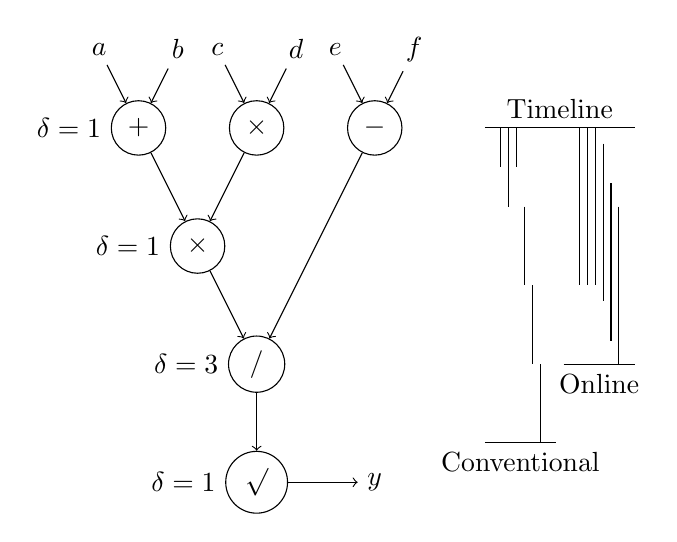
\begin{tikzpicture}
  \path
  (-0.5,5)   node(a) {$a$}
  (0.5,5)    node(b) {$b$}
  (1.0,5)    node(c) {$c$}
  (2,5)      node(d) {$d$}
  (2.5,5)    node(e) {$e$}
  (3.5,5)    node(f) {$f$}

  (0,4)      node[circle,draw,label=left:{$\delta=1$}](p1)  {$+$}
  (1.5,4)    node[circle,draw](p2)                          {$\times$}
  (3,4)      node[circle,draw](p3)                          {$-$}
  (0.75,2.5) node[circle,draw,label=left:{$\delta=1$}](p4)  {$\times$}
  (1.5,1)    node[circle,draw,label=left:{$\delta=3$}](p5)  {$/$}
  (1.5,-0.5) node[circle,draw,label=left:{$\delta=1$}](p6)  {$\surd$}

  (3,-0.5)   node(y) {$y$}
  ;

  \draw[->] (a) -- (p1);
  \draw[->] (b) -- (p1);
  \draw[->] (c) -- (p2);
  \draw[->] (d) -- (p2);
  \draw[->] (e) -- (p3);
  \draw[->] (f) -- (p3);

  \draw[->] (p1) -- (p4);
  \draw[->] (p2) -- (p4);
  \draw[->] (p3) -- (p5);
  \draw[->] (p4) -- (p5);
  \draw[->] (p5) -- (p6);

  \draw[->] (p6) -- (y);

  \draw (4.4,4) -- (6.3,4) node[midway,above]() {Timeline};;
  \draw (4.4,0) -- (5.3,0) node[midway,below]() {Conventional};
  \draw (5.4,1) -- (6.3,1) node[midway,below]() {Online};

  \draw (4.6,4) -- (4.6,3.5);
  \draw (4.7,4) -- (4.7,3);
  \draw (4.8,4) -- (4.8,3.5);
  \draw (4.9,3) -- (4.9,2);
  \draw (5.0,2) -- (5.0,1);
  \draw (5.1,1) -- (5.1,0);

  \draw (5.6,4) -- (5.6,2);
  \draw (5.7,4) -- (5.7,2);
  \draw (5.8,4) -- (5.8,2);
  \draw (5.9,3.8) -- (5.9,1.8);
  \draw (6.0,3.3) -- (6.0,1.3);
  \draw (6.1,3) -- (6.1,1);

\end{tikzpicture}
  \caption{Computing $y=\sqrt{(a+b)cd/(e-f)}$ with serial online operators~\cite{Ercegovac1}}
  \label{Online}
\end{figure}

As illustrated in figure~\ref{Online}, while each individual operation may take longer than its conventional counterpart, online arithmetic can provide a speedup if the operators are chained in serial.
In addition to the tradeoff in time, individual online arithmetic operators also uses more memory.
To perform all computation from the MSD to the LSD, the use of a redundant number system is compulsory.
However, this redundancy also has its advantage in making the operators scalable.
The time required per digit can be made independent of the length of the operands~\cite{Trivedi1}.

A recently proposed architecture allows the precision of online arithmetic to be controlled at runtime~\cite{Zhao1}.
Traditionally, this runtime control was restricted due to the parallel adders present in the multipliers and dividers.
This architecture reuses a fixed-precision adder and stores residues in on-chip RAM.
As such, a single piece of hardware can be used to calculate to any precision, limited only by the size of the on-chip RAM.

The way online arithmetic alleviates the second problem of fixed precision falls out directly from its MSD-first nature.
Suppose the output of a conventional ripple adder is sampled before it has completed its operation.
In this case, the lower digits would have been completed, but the carry would not have reached the higher ones.
This means the error on the result would be significant, as the top bits were still undetermined~\cite{Shi1}.
However, if the output of a parallel online adder is sampled before its completion, the lower bits would be the undetermined ones.
This means the error of the operation would be small.
With overclocking, online arithmetic operators fail gracefully, losing their precision gradually from the lowest bits first.
Thus, it allows for a runtime tradeoff between precision and frequency~\cite{Shi2}.

% REVISIT JD: find better arguments for high radix on FPGA for these two paras
\subsection{High-radix Arithmetic}
Conventional designs of arithmetic operators use binary representations.
The additional concerns of high-radix operators did not provide justifiable improvements as clock speed of processors kept increasing.
In recent years, the clock speed increase effectively ended, and semiconductor dies shrunk to extremely small sizes.
This means the relative processing time available in a clock period increased.
This enabled and drove the desire for accomplishing more per clock cycle, and high-radix arithmetic is one of them.
It has been shown that, high-radix offers power saving and/or reasonable speedups to the arithmetic operations~\cite{Catanzaro1}\cite{Amin1}\cite{Chen1}.

However, the savings are not without trade-offs.
If the radix chosen is not a power of 2, then this trade-off can become unfavourable if the specification requires much I/O and little computation.
This is because overhead of radix conversion would be significant~\cite{Whyte1}.
It is also unwise to use high-radix representations when the numbers are unusually small, thus making the savings offered by the high-radices negligible~\cite{Catanzaro1}.
The radix also cannot be too high, as the time in a clock period is still limited, if there is too many logic gates for the signal to propagate through, it might become the critical path and slow down the overall design.

The construct of FPGAs might make high-radices more attractive than it is on ICs.
As FPGAs contain small fast carry-ripple adders, high-radix adders may be able to exploit them to obtain significant speedups~\cite{Kornerup1}.

\subsection{High-radix Online Arithmetic}
Using high-radix number representations for online arithmetic is a relatively novel concept.
While there has been some research with similar premises~\cite{Lynch1}\cite{Lynch2}, We take a more direct approach with this project by implementing custom operators made for high-radix online arithmetic on an FPGA.
This will provide empirical results on the method, and will hopefully reveal practical insights along the way.

Furthermore, benchmarking this exotic arithmetic system with popular FPGA applications such as neural networks would be interesting, as there is not much precedence for it.


\begin{thebibliography}{1}
% Unused:
% M. D. Ercegovac and T. Lang. Digital Arithmetic

\bibitem{Ahmed1}
  I. Ahmed, S. Zhao, J. Meijers, O. Trescases and V. Betz,
  ``\textit{Automatic BRAM Testing for Robust Dynamic Voltage Scaling for
  FPGAs}'',
  \textit{Int. Conf. on Field-Programmable Logic and Applications},
  2018.

\bibitem{Amin1}
  A Amin, W. Shinwari,
  ``\textit{High-Radix Multiplier-Dividers: Theory, Design, and Hardware}'',
  \textit{IEEE Trans. Comput.}, vol. 1, no.8,
  2008.

\bibitem{Brent1}
  R.P. Brent,
  ``\textit{A Regular Layout for Parallel Adders}'',
  \textit{IEEE Trans. Comput.}, vol. C-31, pp. 260-264,
  1982.

\bibitem{Catanzaro1}
  B. Catanzaro, and B. Nelson,
  ``\textit{Higher Radix Floating-Point Representations for FPGA-Based
  Arithmetic}'',
  \textit{Proceedings of the 51st Annual Design Automation Conference},
  2005.

\bibitem{Chen1}
  L. Chen, F. Lombardi, P. Montuschi, J. Han and W. Liu,
  ``\textit{Design of Approximate High-Radix Dividers by Inexact Binary
  Signed-Digit Addition}'',
  \textit{Proceedings of the on Great Lakes Symposium on VLSI},
  2017.

\bibitem{Duncan1}
  R. Duncan,
  ``\textit{A Survey of Parallel Computer Architectures}'',
  \textit{Computer}, vol. 23, pp. 5-16,
  1990.

\bibitem{Duran1}
  J.W. Duran,
  ``\textit{An Evaluation of Random Testing}'',
  \textit{IEEE Trans. on Software Engineering}, vol. SE-10, no. 4, pp. 438-444,
  1984.

\bibitem{Ercegovac1}
  M.D. Ercegovac,
  ``\textit{On-line Arithmetic: An Overview}'',
  \textit{28th Annual Technical Symposium}, pp. 86-93,
  Internaltional Society for Optics and Photonics,
  1984.

\bibitem{Ercegovac2}
  M.D. Ercegovac, and T. Lang,
  ``\textit{Digital Arithmetic}'',
  Morgan Kaufmann,
  2003.

\bibitem{Hazwani1}
  S. Hazwani, et al,
  ``\textit{Randomness Analysis of Pseudo Random Noise Generator Using 24-bits
  LFSR}'',
  \textit{Fifth Int. Conf. on Intelligent Systems, Modelling and Simulation},
  2014.

\bibitem{Kornerup1}
  P. Kornerup,
  ``\textit{Reviewing High-Radix Signed-Digit Adders}'',
  \textit{IEEE Trans. Comput.}, vol.64, no. 5, pp. 1502-1505,
  2015.

\bibitem{Li1}
  H. Li, J.J. Davis, J. Wickerson and G.A. Constantinides,
  ``\textit{ARCHITECT: Arbitrary-precision Constant-hardware Iterative
  Compute}'',
  \textit{Int. Conf. on Field-Programmable Technology},
  2017.

\bibitem{Lynch1}
  T. Lynch, and M.J. Schulte,
  ``\textit{A High Radix On-line Arithmetic for Credible and Accurate
  Computing}'',
  \textit{Journal of Universal Computer Science}, vol. 1, no. 7, pp. 439-453,
  1995.

\bibitem{Lynch2}
  T. Lynch, and M.J. Schulte,
  ``\textit{Software for High Radix On-line Arithmetic}'',
  \textit{Reliable Computing}, vol. 2, no. 2, pp. 133-138,
  1996.

\bibitem{Srinivas1}
  H.R. Srinivas, and K.K. Parhi,
  ``\textit{High-Speed VLSI Arithmetic Processor Architectures Using Hybrid
  Number Representation}'',
  \textit{J. of VLSI Sign. Process.}, vol. 4. pp. 177-198,
  1992.

\bibitem{Shi1}
  K. Shi, D. Boland, and G.A. Constantinides,
  ``\textit{Accuracy-Performance Tradeoffs on an FPGA through Overclocking}'',
  \textit{Proc. Int. Symp. Field-Programmable Custom Computing Machines},
  pp. 29-36,
  2013.

\bibitem{Shi2}
  K. Shi, D. Boland, E. Stott, S. Bayliss, and G.A. Constantinides,
  ``\textit{Datapath Synthesis for Overclocking: Online Arithmetic for
  Latency-Accuracy Trade-offs}'',
  \textit{Proceedings of the 13th Symposium on Field-Programmable Custom
  Computing Machines},
  pp. 1-6, ACM,
  2014.

\bibitem{Scekic1}
  O. Šćekić
  ``\textit{FPGA Comparative Analysis}'',
  \textit{University of Belgrade},
  2005.

\bibitem{Tenca1}
  A.F. Tenca, and M.D. Ercegovac,
  ``\textit{Design of high-radix digit-slices for on-line computations}'',
  2007.

\bibitem{Trivedi1}
  K.S. Trivedi, and M.D. Ercegovac,
  ``\textit{On-line Algorithms for Division and Multiplication}'',
  \textit{IEEE Trans. Comput.}, vol. C-26, no. 7, pp. 667-680,
  1977.

\bibitem{Whyte1}
  P. Whyte,
  ``\textit{Design and Implementation of High-radix Arithmetic Systems Based
  on the SDNR/RNS Data Representation}''
  \textit{Edith Cowan University},
  1997.

\bibitem{Zhao1}
  Y. Zhao, J. Wickerson, and G.A. Constantinides,
  ``\textit{An Efficient Implementation of Online Arithmetic}'',
  \textit{Int. Conf. on Field-Programmable Technology},
  2016.

% ------------------------------------------------------------------------------

\bibitem{Accellera1}
  Accellera Systems Initiative,
  ``\textit{Universal Verification Methodology 1.2 User’s Guide}'',
  2015.
  % Available at:\\\url{https://accellera.org/images/downloads/standards/uvm/
  % uvm_users_guide_1.2.pdf}.

\bibitem{Altera1}
  Altera Corporation,
  ``\textit{Cyclone V SoC Development Board Reference Manual}'',
  2015.
  % Available at:\\\url{www.intel.com/content/dam/www/programmable/us/en/pdfs/
  % literature/manual/rm_cv_soc_dev_board.pdf}.

\bibitem{Altera2}
  Altera Corporation,
  ``\textit{Memory System Design}'',
  \textit{Embedded Design Handbook},
  2010.
  % Available at:\\\url{www.intel.com/content/dam/www/programmable/us/en/pdfs/
  % literature/hb/nios2/edh_ed51008.pdf}.

\bibitem{Altera3}
  Altera Corporation,
  ``\textit{Introduction to Altmemphy IP}'',
  \textit{External Memory Interface Handbook: Reference Material}, vol. 3,
  2012.
  % Available at:\\\url{www.intel.com/content/dam/www/programmable/us/en/pdfs/
  % literature/hb/external-memory/emi_ddr3_ug.pdf}

\bibitem{Altera4}
  Altera Corporation,
  ``\textit{Phase-Locked Loop Basics, PLL},''.
  % Available at:\\\url{https://www.intel.com/content/www/us/en/programmable/
  % support/support-resources/operation-and-testing/pll-and-clock-management/
  % pll-basics.html}

\bibitem{Altera5}
  Altera Corporation,
  ``\textit{Creating Qsys Components}'',
  2018.
  % Available at:\\\url{https://www.intel.com/content/dam/www/programmable/us/
  % en/pdfs/literature/hb/qts/qsys_components.pdf}.

\bibitem{Altera6}
  Altera Corporation,
  ``\textit{Cyclone V Hard Processor System Technical Reference Manual}'',
  2018.
  % Available at:\\\url{https://www.intel.com/content/dam/www/programmable/us/
  % en/pdfs/literature/hb/cyclone-v/cv_54005.pdf}.

\bibitem{Imperial1}
  Imperial College
  ``\textit{An Ethics Code}'',
  \textit{Imperial College Research Ethics Committee},
  2013.

\bibitem{Intel1}
  Intel Corporation,
  ``\textit{Cyclone V SoC Development Kit and Intel SoC FPGA Embedded
  Development Suite}''.
  % Available at:\\\url{www.intel.com/content/www/us/en/programmable/products/
  % boards_and_kits/dev-kits/altera/kit-cyclone-v-soc.html}.

\bibitem{Intel2}
  Intel Corporation,
  ``\textit{Introduction to Intel FPGA IP Cores}'',
  2018.
  % Available at:\\\url{https://www.intel.com/content/www/us/en/programmable/
  % documentation/mwh1409960636914.html}.

\bibitem{Intel3}
  Intel Corporation,
  ``\textit{Avalon Interface Specifications}'',
  2018.
  % Available at:\\\url{https://www.intel.com/content/dam/www/programmable/us/
  % en/pdfs/literature/manual/mnl_avalon_spec.pdf}.

\bibitem{Rocket1}
  RocketBoards.org,
  ``\textit{GSRD 14.1 User manual}'',
  2015.
  % Available at:\\\url{https://rocketboards.org/foswiki/Documentation/GSRD141}.

\bibitem{Xilinx1}
  Xilinx, Inc,
  ``\textit{Zynq-7000 All Programmable SoC}'',
  2018.
  % Available at:\\\url{www.xilinx.com/support/documentation/
  % product-briefs/zynq-7000-product-brief.pdf}.

\bibitem{Xilinx2}
  Xilinx, Inc,
  ``\textit{ZedBoard (Zynq Evaluation and Development) Hardware User's Guide}'',
  2012.
  % Available at:\\\url{https://reference.digilentinc.com/_media/
  % zedboard:zedboard_ug.pdf}.
\end{thebibliography}

\end{document}